\documentclass{article}
\usepackage{graphicx} % Required for inserting images
\usepackage[english]{babel}
\usepackage{amssymb}
\usepackage{amsthm}
\usepackage{enumitem} 
\usepackage{amsmath}
\usepackage{amsfonts}
\usepackage{tikz}
\usetikzlibrary{matrix}
\usepackage[english]{babel}
\usepackage{mathtools}
\usepackage[a4paper, total={6in, 8in}]{geometry}
\usepackage{cite}
\usepackage{graphicx}
\graphicspath{ {./images/} }


\newtheorem{theorem}{Theorem}[section]
\newtheorem{definition}[theorem]{Definition}
\newtheorem{lemma}[theorem]{Lemma}
\newtheorem{proposition}[theorem]{Proposition}
\newtheorem{corollary}[theorem]{Corollary}
\newtheorem{example}[theorem]{Example}
\newtheorem{remark}[theorem]{Remark}
\newtheorem{exercise}[theorem]{Exercise}


\title{Hatcher solutions}
\author{Saxon Supple}
\date{July 2025}

\begin{document}

\maketitle
\begin{exercise}
Construct an explicit deformation retraction of the torus with one point deleted onto a graph consisting of two circles intersecting in a point, namely, longitude and meridian circles of the torus.
\end{exercise}
\begin{proof}
We can model the torus as the disk $D^2:=\{(x,y)\in\mathbb{R}^2:x^2+y^2\leq 1\}$ where we split the boundary into $4$ equal arcs and identify opposite arcs under the quotient map $q:D^2\to T$. Let $A:=q(\partial D^2)$ be the subspace we wish to retract $T$ onto. Without loss of generality, suppose that we remove the point $(0,0)$. Given a point $x$, we want to send it to $\frac{x}{\|x\|}$ along the line segment from $x$ to $\frac{x}{\|x\|}$. We thus define the homotopy \[F:T\times I\to T:(q(x),t)\mapsto q\left(x(1-t)+\frac{x}{\|x\|}t\right).\] This homotopes between the identity map and a retraction of $T$ onto $A$ while fixing all points of $A$ throughout, and hence is a deformation retraction.
\end{proof}

\begin{exercise}
Construct an explicit deformation retraction of $\mathbb{R}^n\setminus\{0\}$ onto $S^{n-1}$.
\end{exercise}
\begin{proof}
We define a homotopy \[F:\mathbb{R}^n\setminus\{0\}\times I\to S^{n-1}:(x,t)\mapsto x(1-t)+\frac{x}{\|x\|}t.\] This homotopes between the identity map on $\mathbb{R}^n\setminus\{0\}$ and a retraction of $\mathbb{R}^n\setminus\{0\}$ onto $S^{n-1}$, and hence is a deformation retraction.
\end{proof}

\begin{exercise}
\begin{enumerate}
\item[(a)] Show that the composition of homotopy equivalences $X\to Y$ and $Y\to Z$ is a homotopy equivalence $X\to Z$. Deduce that homotopy equivalence is an equivalence relation.
\item[(b)] Show that the relation of homotopy among maps $X\to Y$ is an equivalence relation.
\item[(c)] Show that a map homotopic to a homotopy equivalence is a homotopy equivalence.
\end{enumerate}
\end{exercise}
\begin{proof}
\begin{enumerate}
\item[(a)] Let $\phi:X\to Y$ and $\psi: Y\to Z$ be homotopy equivalences. There then exist homotopy inverses $\phi_1:Y\to X$ and $\psi_1: Z\to Y$ of $\phi$ and $\psi$ respectively.\[(\phi_1\circ\psi_1)\circ(\psi\circ\phi)= \phi_1\circ(\psi_1\circ\psi)\circ\phi\simeq\phi_1\circ\phi\simeq\text{id}_X\] and\[(\psi\circ\phi)\circ(\phi_1\circ\psi_1)=\psi\circ(\phi\circ\phi_1)\circ\psi_1\simeq\psi\circ\psi_1\simeq\text{id}_Z\]so $\psi\circ\phi$ is a homotopy equivalence.
\item[(b)] Let $\phi,\psi,\rho$ be continuous maps from $X$ to $Y$. Clearly $\phi\simeq\phi$. Furthermore, if $F:X\times I\to Y$ is a homotopy from $\phi$ to $\psi$, then $G:X\times I\to Y:(x,t)\mapsto F(x,1-t)$ is a homotopy from $\psi$ to $\phi$. Finally, let $A:X\times I\to Y$ be a homotopy from $\phi$ to $\psi$ and let $B:X\times I\to Y$ be a homotopy from $\psi$ to $\rho$. We define a map $C:X\times I\to Y$ by \[C(x,t)=\begin{cases}
    A(x,2t)\text{ if }0\leq t\leq \frac{1}{2}\\B(x,2t-1)\text{ if }\frac{1}{2}<t\leq 1.
\end{cases}\]$X\times[0,\frac{1}{2}]$ and $X\times[\frac{1}{2},1]$ are both closed subsets of $X\times I$ with $X\times[0,\frac{1}{2}]\cup X\times[\frac{1}{2},1]=X\times I$. Furthermore, $C_{|{X\times[0,\frac{1}{2}]}}$ and $C_{|{X\times[\frac{1}{2},1]}}$ are both continuous with respect to the induced topologies on $X\times[0,\frac{1}{2}]$ and $X\times[\frac{1}{2},1]$ respectively. Hence, $C$ is continuous on $X\times I$ and is thus a homotopy from $\phi$ to $\rho$.
\item[(c)] Let $\phi:X\to Y$ be a homotopy equivalence with homotopy inverse $\psi:Y\to X$. Let $\phi_1:X\to Y$ be homotopic to $\phi$. Then \[\phi_1\circ\psi\simeq\phi\circ\psi\simeq\text{id}_Y\] and \[\psi\circ\phi_1\simeq\psi\circ\phi\simeq\text{id}_X.\] Hence $\phi_1$ is a homotopy equivalence.
\end{enumerate}
\end{proof}

\begin{exercise}
A $\textbf{deformation retraction in the weak sense}$ of a space $X$ to a subspace $A$ is a homotopy $f_t:X\to X$ such that $f_0=\mathbb{1}$, $f_1(X)\subset A$, and $f_t(A)\subset A$ for all $t$. Show that if $X$ deformation retracts to $A$ in this weak sense, then the inclusion $A\hookrightarrow X$ is a homotopy equivalence.
\end{exercise}
\begin{proof}
Let $\iota:A\to X$ denote the inclusion $A\hookrightarrow X$. Define $\phi:X\to A:x\mapsto f_1(x)$, which is well-defined since $f_1(X)\subset A$. Then \[\phi\circ\iota={f_1}_{|A}\simeq {f_0}_{|A}=\text{id}_A.\]This is a valid homotopy of maps $A\to A$ since $f_1(A)\subset A\forall t$. Furthermore,\[\iota\circ\phi=f_1\simeq\text{id}_X.\] Hence $\iota$ is a homotopy equivalence with homotopy inverse $\phi$.
\end{proof}

\begin{exercise}
Show that if a space $X$ deformation retracts to a point $x\in X$, then for each neighbourhood $U$ of $x$ in $X$ there exists a neighbourhood $V\subset U$ of $x$ such that the inclusion map $V\hookrightarrow U$ is nullhomotopic.
\end{exercise}
\begin{proof}
Without loss of generality, let $U$ be an open neighbourhood of $x$. Define \[F:X\times I\to X:(y,t)\mapsto f_t(y)\] and let $A:=F^{-1}(U)$. $A$ is an open set containing the slice $\{x\}\times I$, so by the Tube Lemma there exists a tube $V\times I\subset X\times I$, where $V$ is open and contains $x$. Furthermore, $V\times I\subset A$, so $V$ consists only of points in $U$ (since $V\times\{0\}\subset U\times\{0\}$) which stay in $U$ throughout the homotopy $f_t$. Let $\iota:V\hookrightarrow U$ be the inclusion map $V\hookrightarrow U$. Then $f_t:X\to X$ restricts to a homotopy ${f_t}_{|V}:V\to U$ and hence $\iota\simeq {f_1}_{|V}$, where ${f_1}_{|V}$ is the constant map, so $\iota$ is nullhomotopic.
\end{proof}

\begin{exercise}
\begin{enumerate}
\item[(a)] Let $X$ be the subspace of $\mathbb{R}^2$ consisting of the horizontal segment $[0,1]\times\{0\}$ together with all the vertical segments $\{r\}\times[0,1-r]$ for $r$ a rational number in $[0,1]$. Show that $X$ deformation retracts to any point in the segment $[0,1]\times\{0\}$, but not to any other point.
\item[(b)] Let $Y$ be the subspace of $\mathbb{R}^2$ that is the union of an infinite number of copies of $X$ arranged as in the figure below. Show that $Y$ is contractible but does not deformation retract onto any point.

\includegraphics[scale=0.5]{Screenshot 2025-07-20 at 19-46-35 AT.dvi - AT.pdf.png}
\item[(c)] Let $Z$ be the zigzag subspace of $Y$ homeomorphic to $\mathbb{R}$ indicated by the heavier line. Show there is a deformation retraction in the weak sense of $Y$ onto $Z$, but no true deformation retraction.
\end{enumerate}
\end{exercise}
\begin{proof}
\begin{enumerate}
\item[(a)] We define a homotopy \[f_t:X\to X:(a,b) \mapsto (a,b(1-t)).\] $f_t$ fixes $[0,1]\times\{0\}$, $f_0=\text{id}_X$ and $f_1$ is a retraction from $X$ to $[0,1]\times\{0\}$, so $f_t$ is a deformation retraction. Hence $[0,1]\times\{0\}$ is a deformation retract of $X$. Any point in $[0,1]\times\{0\}$ is then clearly a deformation retract of $[0,1]\times\{0\}$, so  $X$ deformation retracts to any point in $[0,1]\times\{0\}$ by transitivity. Now suppose $X$ deformation retracts to some other point $x\in X$. We can then find a neighbourhood $U$ of $x$ of the form $B_\epsilon(x)\cap X$ for some $\epsilon > 0$, which does not contain $[0,1]\times\{0\}$. However, $U$ is not path-connected, so there does not exist a neighbourhood $V\subset U$ of $x$ such that the inclusion map $V\hookrightarrow U$ is nullhomotopic; a contradiction.
\item[(b)] Define a homotopy $f_t:Y\to Y$ where $f_t(y)$ sends $y$ a distance of $t$ to the right along $Y$. Then $f_0=\text{id}_Y$ and $f_1(Y)=Z$, where $Z$ is the zigzag subspace of $Y$. $Z$ is contractible, being homeomorphic to $\mathbb{R}$, and hence there exists a homotopy $h_t:Z\to Z$ from $\text{id}_Z$ to a constant function. We can then define a homotopy $F_t:Y\to Y$ of $\text{id}_Y$ to a constant map by\[F_t(y)=\begin{cases}
    f_{2t}(y)\text{ if }0\leq t\leq\frac{1}{2},
    \\h_{2t-1}\circ f_1(y)\text{ if }\frac{1}{2}< t\leq 1.
\end{cases}\]

Now suppose $Y$ deformation retracts onto a point $y$. We can then find a sufficiently small open neighbourhood $U$ of $y$ such that for every neighbourhood $V\subset U$ of $y$, $U$ is not path-connected, and hence the inclusion map $V\hookrightarrow U$ is not nullhomotopic; a contradiction. Hence $Y$ does not deformation retract onto a point $y$.
\item[(c)] Since $Z$ deformation retracts onto a point, if there were a deformation retract of $Y$ onto $Z$, then there would be a deformation retract of $Y$ onto a point. However, (b) showed that this is not the case, and hence $Y$ does not deformation retract onto $Z$. However, the homotopy $f_t$ defined in (b) is a weak deformation retract of $Y$ onto $Z$.
\end{enumerate}
\end{proof}

\begin{exercise}
Fill in the details in the following construction from
[Edwards 1999] of a compact space $Y\subset\mathbb{R}^3$ with the
same properties as the space $Y$ in Exercise $6$, that is, $Y$
is contractible but does not deformation retract to any
point. To begin, let $X$ be the union of an infinite sequence of cones on the Cantor set arranged end-to-end,
as in the figure. Next, form the one-point compactification of $X\times\mathbb{R}$. This embeds in $\mathbb{R}^3$ as a closed disk with curved ‘fins’ attached along circular arcs, and with the one-point compactification of $X$ as a cross-sectional slice.
The desired space $Y$ is then obtained from this subspace of $\mathbb{R}^3$ by wrapping one more
cone on the Cantor set around the boundary of the disk.

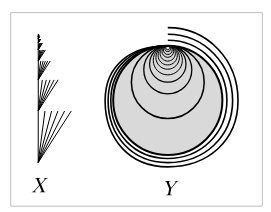
\includegraphics[scale=0.5]{Screenshot 2025-07-21 at 17-47-12 AT.dvi - AT.pdf.png}
\end{exercise}

\begin{exercise}
For $n>2$, construct an $n$-room analog of the house with two rooms.
\end{exercise}

\begin{exercise}
Show that a retract of a contractible space is contractible.
\end{exercise}
\begin{proof}
Let $X$ be a contractible space with $A$ a retract of $X$. Let $f_t:X\to X$ be a homotopy from $\text{id}_X$ to a constant map, and let $r:X\to A$ be a retraction of $X$ onto $A$. $r\circ {f_0}_{|A}=\text{id}_A$ and $r\circ {f_1}_{|A}$ is constant due to ${f_1}_{|A}$ being constant. Hence $\text{id}_A$ is homotopic to a constant map so $A$ is contractible.
\end{proof}

\begin{exercise}
Show that a space $X$ is contractible iff every map $f:X\to Y$, for arbitrary $Y$, is
nullhomotopic. Similarly, show $X$ is contractible iff every map $f:Y\to X$ is nullhomotopic.
\end{exercise}
\begin{proof}
$(\impliedby)$: Let $Y=X$ and $f=\text{id}_X$. Then $\text{id}_X$ is nullhomotopic so $X$ is contractible.

$(\implies)$: Let $g_t:X\to X$ be a homotopy from $\text{id}_X$ to a constant map. Then define a homotopy $h_t:X\to Y$ by $h_t(x)=f\circ g_t(x)$. This is a homotopy between $f$ and a constant map, so $f$ is nullhomotopic.

$(\impliedby)$: Again, let $Y=X$ and $f=\text{id}_X$.

$(\implies)$: $g_t\circ f$ is a homotopy from $f$ to a constant map so $f$ is nullhomotopic.
\end{proof}

\begin{exercise}
Show that $f:X\to Y$ is a homotopy equivalence if there exist maps $g,h:Y\to X$ such that $fg\simeq\mathbb{1}$ and $hf\simeq\mathbb{1}$. More generally, show that $f$ is a homotopy equivalence if $fg$ and $hf$ are homotopy equivalences.
\end{exercise}
\begin{proof}
$fgfh,gfhf$
$fhfg,hfgf$
Let $\phi=h\circ f\circ g:Y\to X$. Then\[f\circ\phi=f\circ(h\circ f\circ g)=f\circ(h\circ f)\circ g\simeq f\circ g\simeq\mathbb{1}\] and\[\phi\circ f=(h\circ f\circ g)\circ f=h\circ(f\circ g)\circ f\simeq h\circ f\simeq\mathbb{1}\] so $\phi$ is a homotopy inverse of $f$ so $f$ is a homotopy equivalence.

Let $g_1$ and $h_1$ be the homotopy inverses of $fg$ and $hf$ respectively. We then have that $f(gg_1)\simeq\mathbb{1}$ and $(h_1h)f\simeq\mathbb{1}$, and hence $f$ is a homotopy equivalence with homotopy inverse $h_1hfgg_1$.
\end{proof}

\end{document}
